\qrchapter{https://forgottenpillar.com/rsc/en-fp-chapter14}{Adventist pioneers and the Trinity doctrine}


\qrchapter{https://forgottenpillar.com/rsc/en-fp-chapter14}{Les pionniers adventistes et la doctrine de la Trinité}


Sister White wrote that early Adventist pioneers \egwinline{are to bear their testimony as to what constitutes the truth for this time}[Lt329-1905.18; 1905][https://egwwritings.org/read?panels=p8455.24] because \egwinline{they have learned to avoid errors and dangers, and are they not then competent to give wise counsel}[7T 287.3; 1902][https://egwwritings.org/read?panels=p117.1637]? In their writings, we see their unanimous views regarding the \emcap{personality of God}, and that they have avoided the Trinitarian error. There is much to write about this topic because the Adventist pioneers left a lot of material dealing directly or indirectly with the doctrine of Trinity. But we will look at some of the testimonies from James White and brother Loughborough because we have read some of their articles on the \emcap{personality of God}. Also, we will compare their testimony with the Spirit of Prophecy as we have done so far.


Sœur White a écrit que les premiers pionniers adventistes \egwinline{doivent porter leur témoignage quant à ce qui constitue la vérité pour ce temps}[Lt329-1905.18; 1905][https://egwwritings.org/read?panels=p8455.24] parce qu’\egwinline{ils ont appris à éviter les erreurs et les dangers, et ne sont-ils pas alors compétents pour donner de sages conseils}[7T 287.3; 1902][https://egwwritings.org/read?panels=p117.1637] ? Dans leurs écrits, nous voyons leurs vues unanimes concernant la \emcap{personnalité de Dieu}, et qu'ils ont évité l'erreur trinitaire. Il y a beaucoup à écrire sur ce sujet parce que les pionniers adventistes ont laissé beaucoup de matériel traitant directement ou indirectement de la doctrine de la Trinité. Mais nous examinerons quelques-uns des témoignages de James White et du frère Loughborough parce que nous avons lu certains de leurs articles sur la \emcap{personnalité de Dieu}. De plus, nous comparerons leur témoignage avec l'Esprit de Prophétie comme nous l'avons fait jusqu'à présent.


James White, in the Review and Herald, listed \others{some of \textbf{the popular fables} of the age}”, saying: “\others{Here we might mention \textbf{the Trinity, which \underline{does away the personality of God, and of his Son Jesus Christ,} }and of sprinkling or pouring instead of being ‘buried with Christ in baptism,’ ‘planted in the likeness of his death:’ but we pass from these \textbf{fables }to notice one that is held sacred by nearly all professed Christians, both Catholic and Protestant. It is, the change of the Sabbath of the fourth commandment from the seventh to the first day of the week.}[James S. White, Review \& Herald, December 11, 1855, p. 85.15][http://documents.adventistarchives.org/Periodicals/RH/RH18551211-V07-11.pdf]


James White, dans la Review and Herald, a énuméré \others{quelques-unes des \textbf{fables populaires} de l'époque}, disant : « \others{Ici nous pourrions mentionner \textbf{la Trinité, qui \underline{supprime la personnalité de Dieu, et de son Fils Jésus-Christ,} }et l'aspersion ou le versement au lieu d'être ‘ensevelis avec Christ par le baptême’, ‘ayant été faits une même plante avec lui par la conformité à sa mort’ : mais nous passons de ces \textbf{fables }pour remarquer une qui est tenue pour sacrée par presque tous les chrétiens professés, catholiques et protestants. C'est le changement du sabbat du quatrième commandement du septième au premier jour de la semaine.} »[James S. White, Review \& Herald, December 11, 1855, p. 85.15][http://documents.adventistarchives.org/Periodicals/RH/RH18551211-V07-11.pdf]


What does James White mean when he says that the Trinity \others{does away with the personality of God, and of his Son Jesus Christ}? In Day Star, he wrote:


Que veut dire James White quand il dit que la Trinité \others{supprime la personnalité de Dieu, et de son Fils Jésus-Christ} ? Dans Day Star, il a écrit :


\others{…a certain class who \textbf{deny the only Lord God and our Lord Jesus Christ}. This class can be no other than those who \textbf{spiritualize away the existence of the Father and the Son}, \textbf{as \underline{two distinct}, \underline{literal}, \underline{tangible persons}}, also a literal Holy city and throne of David… The way spiritualizers this way have disposed of or \textbf{denied the only Lord God and our Lord Jesus Christ is first using \underline{the old unscriptural trinitarian creed}}, viz, that Jesus Christ is the eternal God, though they have not one passage to support it, while we have plain scripture testimony in abundance \textbf{that He is the Son of the eternal God.}}[James White, Day Star, Jan 24, 1846][https://m.egwwritings.org/en/book/741.25\#27]


\others{…une certaine classe qui \textbf{nie le seul Seigneur Dieu et notre Seigneur Jésus-Christ}. Cette classe ne peut être autre que ceux qui \textbf{spiritualisent l'existence du Père et du Fils}, \textbf{comme \underline{deux personnes distinctes}, \underline{littérales}, \underline{tangibles}}, aussi une ville sainte littérale et le trône de David… La façon dont les spiritualistes ont disposé ou \textbf{nié le seul Seigneur Dieu et notre Seigneur Jésus-Christ est d'abord en utilisant \underline{l'ancien credo trinitaire non scripturaire}}, à savoir, que Jésus-Christ est le Dieu éternel, bien qu'ils n'aient pas un seul passage pour le soutenir, tandis que nous avons un témoignage scripturaire clair en abondance \textbf{qu'Il est le Fils du Dieu éternel.}}[James White, Day Star, Jan 24, 1846][https://m.egwwritings.org/en/book/741.25\#27]


Doing away with the personality of God and His Son is accomplished by denying Them as two distinct, literal, and tangible persons. The doctrine on the personality of God teaches that the Father has a literal, \textit{tangible} person.


Supprimer la personnalité de Dieu et de Son Fils s'accomplit en Les niant comme deux personnes distinctes, littérales et tangibles. La doctrine sur la personnalité de Dieu enseigne que le Père a une personne littérale, \textit{tangible}.


In the Adventist Review and Sabbath Herald article from April 4, 1854, James White listed 10 points of \textit{Catholic reasons for keeping Sunday}”, where he said that the Sunday \others{is a day dedicated by the apostles to \textbf{the honor of the most Holy Trinity}}[The Advent Review, and Sabbath Herald, vol. 5 April 4, 1854, p. 86][https://egwwritings.org/read?panels=p1643.2867]. Here we also see the harmony between J. B. Frisbie and James White in their view that the Sabbath is dedicated to the biblical God expressed in the first point of the \emcap{Fundamental Principles}, and Sunday is dedicated to the trinity God. The main problem with the Trinity doctrine is that it \others{does away the personality of God, and of his Son Jesus Christ}. In Life Incidents, he wrote more about why this is so.


Dans l'article de l'Adventist Review and Sabbath Herald du 4 avril 1854, James White a énuméré 10 points de \textit{raisons catholiques pour garder le dimanche}, où il a dit que le dimanche \others{est un jour dédié par les apôtres à \textbf{l'honneur de la très Sainte Trinité}}[The Advent Review, and Sabbath Herald, vol. 5 April 4, 1854, p. 86][https://egwwritings.org/read?panels=p1643.2867]. Ici nous voyons aussi l'harmonie entre J. B. Frisbie et James White dans leur vue que le sabbat est dédié au Dieu biblique exprimé dans le premier point des \emcap{Principes Fondamentaux}, et le dimanche est dédié au dieu trinité. Le problème principal avec la doctrine de la Trinité est qu'elle \others{supprime la personnalité de Dieu, et de son Fils Jésus-Christ}. Dans Life Incidents, il a écrit davantage sur pourquoi il en est ainsi.


\others{\textbf{Jesus prayed that his disciples might be one as he was \underline{one with his Father}}. \textbf{This prayer did not contemplate one disciple with twelve heads, but twelve disciples, made one in object and effort in the cause of their Master}. \textbf{\underline{Neither are the Father and the Son parts of the ‘three-one God.}}’\footnote{The same quotation is found in James White’s book “\textit{The Law and the Gospel}” with one difference. He states, “\textit{Neither are the Father and the Son parts of \underline{one being}}”; in “\textit{Life Incidents}”, he wrote “parts of the ‘\underline{three-one God}’”. See \href{https://egwwritings.org/?ref=en_LAGO.1.2&para=1492.10}{James S. White, The Law and the Gospel p. 1.2}.} \textbf{\underline{They are two distinct beings}}, \textbf{yet one in the design and accomplishment of redemption}. The redeemed, from the first who shares in the great redemption, to the last, all ascribe the honour, and glory, and praise, of their salvation, to \textbf{both God and the Lamb}.}[James S. White, Life Incidents, p.343.2][https://egwwritings.org/read?panels=p1462.1743]


\others{\textbf{Jésus a prié pour que ses disciples soient un comme il était \underline{un avec son Père}}. \textbf{Cette prière n'envisageait pas un disciple avec douze têtes, mais douze disciples, rendus un dans l'objectif et l'effort dans la cause de leur Maître}. \textbf{\underline{Le Père et le Fils ne sont pas non plus des parties du ‘Dieu trois-en-un.}}’\footnote{La même citation se trouve dans le livre de James White « \textit{The Law and the Gospel} » avec une différence. Il déclare, « \textit{Le Père et le Fils ne sont pas non plus des parties d’\underline{un seul être}} » ; dans « \textit{Life Incidents} », il a écrit « parties du ‘\underline{Dieu trois-en-un}’ ». Voir \href{https://egwwritings.org/?ref=en_LAGO.1.2&para=1492.10}{James S. White, The Law and the Gospel p. 1.2}.} \textbf{\underline{Ils sont deux êtres distincts}}, \textbf{pourtant un dans la conception et l'accomplissement de la rédemption}. Les rachetés, depuis le premier qui partage la grande rédemption, jusqu'au dernier, tous attribuent l'honneur, et la gloire, et la louange, de leur salut, à \textbf{la fois à Dieu et à l'Agneau}.}[James S. White, Life Incidents, p.343.2][https://egwwritings.org/read?panels=p1462.1743]


Sister White wrote similarly regarding Christ’s prayer:


Sœur White a écrit de manière similaire concernant la prière du Christ :


\egw{The burden of that prayer was that His disciples might be \textbf{one as He was one with the Father}; the oneness so close that, \textbf{although \underline{two distinct beings}}, there was \textbf{perfect unity of spirit, purpose, and action}. The mind of the Father was the mind of the Son.}[Lt1-1882.1; 1882][https://egwwritings.org/read?panels=p4120.5]


\egw{Le fardeau de cette prière était que Ses disciples puissent être \textbf{un comme Il était un avec le Père} ; l'unité si étroite que, \textbf{bien que \underline{deux êtres distincts}}, il y avait \textbf{une parfaite unité d'esprit, de but et d'action}. L'esprit du Père était l'esprit du Fils.}[Lt1-1882.1; 1882][https://egwwritings.org/read?panels=p4120.5]


\egw{\textbf{The unity that exists between Christ and His disciples \underline{does not destroy the personality of either}}. They are one in purpose, in mind, in character, \textbf{but \underline{not in person}}. \textbf{It is thus that God and Christ are one}.}[MH, 421 422; 1905][https://egwwritings.org/read?panels=p135.2177]


\egw{\textbf{L'unité qui existe entre Christ et Ses disciples \underline{ne détruit pas la personnalité de l'un ou de l'autre}}. Ils sont un dans le but, dans l'esprit, dans le caractère, \textbf{mais \underline{pas en personne}}. \textbf{C'est ainsi que Dieu et Christ sont un}.}[MH, 421 422; 1905][https://egwwritings.org/read?panels=p135.2177]


The Father and the Son do not comprise one person nor being. The Father and the Son are one, just as Christ and His disciples are one—one in spirit, purpose, mind, and character.


Le Père et le Fils ne constituent pas une seule personne ni un seul être. Le Père et le Fils sont un, tout comme Christ et Ses disciples sont un—un en esprit, en but, en pensée et en caractère.


Many Adventist trinitarian scholars charge James White and other early pioneers for arianism or semi-arianism, claiming that they made Christ inferior to the Father. This is not true. Let us read the testimony of James White on this matter.


De nombreux érudits adventistes trinitaires accusent James White et d'autres premiers pionniers d'arianisme ou de semi-arianisme, prétendant qu'ils ont rendu Christ inférieur au Père. Ce n'est pas vrai. Lisons le témoignage de James White sur cette question.


\others{Paul affirms of \textbf{the Son of God that he was in the form of God}, and that \textbf{\underline{he was equal with God}}. ‘\textbf{Who being in the form of God thought it not robbery to be \underline{equal with God}}.’ Phil. 2:6. The reason why it is not robbery for the Son \textbf{to be equal with the Father is the fact that he is equal}. If the Son is not equal with the Father, then it is robbery for him to rank himself with the Father.}


\others{Paul affirme du \textbf{Fils de Dieu qu'il était en forme de Dieu}, et qu’\textbf{\underline{il était égal à Dieu}}. ‘\textbf{Lequel étant en forme de Dieu, n'a point regardé comme une usurpation d'être \underline{égal à Dieu}}.’ Phil. 2:6. La raison pour laquelle ce n'est pas une usurpation pour le Fils \textbf{d'être égal au Père est le fait qu'il est égal}. Si le Fils n'est pas égal au Père, alors c'est une usurpation pour lui de se classer avec le Père.}


\othersnogap{\textbf{\underline{The inexplicable trinity that makes the godhead three in one and one in three, is bad enough}}; \textbf{but that ultra Unitarianism that makes Christ inferior to the Father is worse}. Did God say to an inferior, Let us make man in our image?’}[James S. White, The Advent Review and Sabbath Herald, November 29, 1877, p. 171][https://documents.adventistarchives.org/Periodicals/RH/RH18771129-V50-22.pdf]


\othersnogap{\textbf{\underline{La trinité inexplicable qui fait de la divinité trois en un et un en trois, est assez mauvaise}}; \textbf{mais cet ultra-unitarisme qui rend Christ inférieur au Père est pire}. Dieu a-t-il dit à un inférieur, Faisons l'homme à notre image ?’}[James S. White, The Advent Review and Sabbath Herald, November 29, 1877, p. 171][https://documents.adventistarchives.org/Periodicals/RH/RH18771129-V50-22.pdf]


The problem of the Adventist trinitarian scholars lies in that they themselves cannot completely explain Christ’s divinity other than through the Trinitarian paradigm. Adventist pioneers did believe in Christ’s full divinity but they rejected the Trinity because it destroys the \emcap{personality of God}. \others{The inexplicable trinity that makes the godhead three in one and one in three, \textbf{is bad enough}}. Below is another statement from James White where he compared Seventh-day Adventist with Seventh-day Baptist belief. Seventh-day Adventists did not believe in the Trinity unlike Seventh-day Baptists. James White mentioned that, regarding the divinity of Christ, Seventh-day Adventists hold so nearly with the trinitarian Seventh-day Baptists that they apprehend no trial there.


Le problème des érudits adventistes trinitaires réside dans le fait qu'ils ne peuvent eux-mêmes expliquer complètement la divinité de Christ autrement que par le paradigme trinitaire. Les pionniers adventistes croyaient en la pleine divinité de Christ mais ils rejetaient la Trinité parce qu'elle détruit la \emcap{personnalité de Dieu}. \others{La trinité inexplicable qui fait de la divinité trois en un et un en trois, \textbf{est assez mauvaise}}. Voici une autre déclaration de James White où il comparait la croyance des Adventistes du Septième Jour avec celle des Baptistes du Septième Jour. Les Adventistes du Septième Jour ne croyaient pas en la Trinité contrairement aux Baptistes du Septième Jour. James White a mentionné que, concernant la divinité de Christ, les Adventistes du Septième Jour adhèrent si étroitement aux Baptistes du Septième Jour trinitaires qu'ils n'appréhendent aucune épreuve là.


\others{\textbf{The principal difference between the two bodies is the immortality question}. \textbf{The S. D. Adventists hold \underline{the divinity of Christ so nearly with the trinitarian}, that we apprehend no trial here}. And as the practical application of the subject of the Gifts of the Spirit to our people and to our work is better understood by our S. D. Baptist brethren, they manifest less concern for us on this account.}[James S. White, The Advent Review and Sabbath Herald, October 12, 1876, p. 116][https://documents.adventistarchives.org/Periodicals/RH/RH18761012-V48-15.pdf]


\others{\textbf{La principale différence entre les deux corps est la question de l'immortalité}. \textbf{Les Adventistes du S. J. tiennent \underline{la divinité de Christ si étroitement avec les trinitaires}, que nous n'appréhendons aucune épreuve ici}. Et comme l'application pratique du sujet des Dons de l'Esprit à notre peuple et à notre œuvre est mieux comprise par nos frères Baptistes du S. J., ils manifestent moins d'inquiétude pour nous à ce sujet.}[James S. White, The Advent Review and Sabbath Herald, October 12, 1876, p. 116][https://documents.adventistarchives.org/Periodicals/RH/RH18761012-V48-15.pdf]


This evidence should raise questions to each Adventist trinitarian scholar. How could it be that the Adventist pioneers adhere to the divinity of Christ as trinitarians did, yet rejected the Trinity doctrine? In which way was Christ fully divine, if He was not part of an amalgamated three-in-one God? The answer is simple and completely Biblical. Christ is fully divine, just as His Father, because He was begotten in the express image of the Father’s person; thus, He inherited complete divine nature from His Father.


Cette preuve devrait soulever des questions à chaque érudit adventiste trinitaire. Comment se fait-il que les pionniers adventistes adhéraient à la divinité de Christ comme le faisaient les trinitaires, tout en rejetant la doctrine de la Trinité ? De quelle manière Christ était-il pleinement divin, s'Il ne faisait pas partie d'un Dieu amalgamé trois-en-un ? La réponse est simple et complètement biblique. Christ est pleinement divin, tout comme Son Père, parce qu'Il a été engendré à l'empreinte de la personne du Père ; ainsi, Il a hérité la nature divine complète de Son Père.


\egw{A complete offering has been made; for ‘God so loved the world, that he gave his only-begotten Son,’—\textbf{not a son by creation}, as were the angels, nor a son by adoption, as is the forgiven sinner, but \textbf{a Son \underline{begotten} in the express image of the Father’s person}, and in all the brightness of his majesty and glory, \textbf{one equal with God} in authority, dignity, and \textbf{divine perfection}. \textbf{In him dwelt all the fullness of the Godhead bodily}.}[ST May 30, 1895, par. 3; 1895][https://egwwritings.org/read?panels=p820.12891]


\egw{Une offrande complète a été faite ; car ‘Dieu a tant aimé le monde qu'il a donné son Fils unique,’—\textbf{pas un fils par création}, comme l'étaient les anges, ni un fils par adoption, comme l'est le pécheur pardonné, mais \textbf{un Fils \underline{engendré} à l'empreinte de la personne du Père}, et dans toute la splendeur de sa majesté et de sa gloire, \textbf{un égal à Dieu} en autorité, dignité, et \textbf{perfection divine}. \textbf{En lui habitait toute la plénitude de la Divinité corporellement}.}[ST May 30, 1895, par. 3; 1895][https://egwwritings.org/read?panels=p820.12891]


Christ's complete divinity is not based on an amalgamated \emcap{personality of God}, but rather on His Sonship with the Father. The Bible never refers to Christ with the term “\textit{one God}”—only the Father is referred to with the term “\textit{one God}”\footnote{John 17:3; 1. Corinthians 8:6; 1. Timothy 2:5; Ephesians 4:6} \footnote{We study Christ’s complete divinity in-depth  in the second book of the Forgotten Pillar Project - “\textit{Rediscovering the Pillar}”}. Jesus, the Son of God, is fully divine but is not referred to as \others{\textbf{one God}, \textbf{a personal, spiritual being}} in the first point of the \emcap{Fundamental Principles}.


La divinité complète de Christ n'est pas basée sur une \emcap{personnalité de Dieu} amalgamée, mais plutôt sur Sa Filiation avec le Père. La Bible ne se réfère jamais à Christ avec le terme “\textit{un seul Dieu}”—seul le Père est désigné par le terme “\textit{un seul Dieu}”\footnote{Jean 17:3; 1 Corinthiens 8:6; 1 Timothée 2:5; Éphésiens 4:6} \footnote{Nous étudions la divinité complète de Christ en profondeur dans le deuxième livre du Projet du Pilier Oublié - “\textit{Redécouvrir le Pilier}”}. Jésus, le Fils de Dieu, est pleinement divin mais n'est pas désigné comme \others{\textbf{un seul Dieu}, \textbf{un être personnel et spirituel}} dans le premier point des \emcap{Principes Fondamentaux}.


\egw{The Lord Jesus Christ, the only begotten Son of the Father, \textbf{is truly God in infinity, \underline{but not in personality}}.}[Ms116-1905.19; 1905][https://egwwritings.org/read?panels=p10633.25]


\egw{Le Seigneur Jésus-Christ, le seul Fils engendré du Père, \textbf{est vraiment Dieu dans l'infinité, \underline{mais pas dans la personnalité}}.}[Ms116-1905.19; 1905][https://egwwritings.org/read?panels=p10633.25]


Brother J. N. Loughborough was asked to answer the question, \others{What serious objection is there to the doctrine of the Trinity?}[The question was asked by Brother W. W. Giles and it was sent to James S. White, who forwarded the question to Brother John N. Loughborough.]. As we read his answer, let us try to understand some of the reasons why the early pioneers did not adhere to this doctrine.


On a demandé à frère J. N. Loughborough de répondre à la question, \others{Quelle objection sérieuse y a-t-il à la doctrine de la Trinité ?}[La question a été posée par frère W. W. Giles et elle a été envoyée à James S. White, qui a transmis la question à frère John N. Loughborough.]. En lisant sa réponse, essayons de comprendre certaines des raisons pour lesquelles les premiers pionniers n'adhéraient pas à cette doctrine.


\others{There are many objections which we might urge, but on account of our limited space we shall reduce them to the three following: \textbf{1. It is contrary to common sense. 2. It is contrary to scripture. 3. Its origin is Pagan and fabulous.}}


\others{Il y a de nombreuses objections que nous pourrions soulever, mais en raison de notre espace limité, nous les réduirons aux trois suivantes : \textbf{1. Elle est contraire au bon sens. 2. Elle est contraire à l'Écriture. 3. Son origine est païenne et fabuleuse.}}


\othersnogap{These positions we will remark upon briefly in their order. And 1. \textbf{It is not very consonant with common sense to talk of three being one, and one being three}. \textbf{Or as some express it, calling God ‘the Triune God,’ or ‘the three-one-God.’} \textbf{If Father, Son, and Holy Ghost are each God, it would be three Gods; for three times one is not one, but three}. \textbf{\underline{There is a sense in which they are one, but not one person, as claimed by Trinitarians}}}.


\othersnogap{Nous commenterons brièvement ces positions dans leur ordre. Et 1. \textbf{Il n'est pas très conforme au bon sens de parler de trois étant un, et un étant trois}. \textbf{Ou comme certains l'expriment, appelant Dieu « le Dieu Trinitaire », ou « le Dieu trois-en-un ».} \textbf{Si le Père, le Fils et le Saint-Esprit sont chacun Dieu, ce serait trois Dieux ; car trois fois un n'est pas un, mais trois}. \textbf{\underline{Il y a un sens dans lequel ils sont un, mais pas une personne, comme le prétendent les Trinitaires}}}.


\othersnogap{2. \textbf{It is contrary to Scripture}. \textbf{Almost any portion of the New Testament we may open which has occasion to speak of the Father and Son, represents them as two distinct persons}. \textbf{\underline{The seventeenth chapter of John is alone sufficient to refute the doctrine of the Trinity}}. \textbf{Over forty times in that one chapter Christ speaks of his Father as a person distinct from himself}. His Father was in heaven and he upon earth. The Father had sent him. Given to him those that believed. He was then to go to the Father.\textbf{ And in this very testimony he shows us in what consists the oneness of the Father and Son}.\textbf{\underline{ It is the same as the oneness of the members of Christ’s church}}. ‘\textbf{That \underline{they} all may be one; \underline{as} thou, Father, art in me, and I in thee, \underline{that they also} may be one in us}; that the world may believe that thou hast sent me. And the \textbf{glory which thou gavest me I have given them}; that \textbf{they may be one}, \textbf{even as we are one.}’ \textbf{Of one heart and one mind}. \textbf{Of one purpose} in all the plan devised for man’s salvation. \textbf{\underline{Read the seventeenth chapter of John, and see if it does not completely upset the doctrine of the Trinity}}.}


\othersnogap{2. \textbf{Elle est contraire à l'Écriture}. \textbf{Presque toute portion du Nouveau Testament que nous pouvons ouvrir qui a l'occasion de parler du Père et du Fils, les représente comme deux personnes distinctes}. \textbf{\underline{Le dix-septième chapitre de Jean est à lui seul suffisant pour réfuter la doctrine de la Trinité}}. \textbf{Plus de quarante fois dans ce seul chapitre, Christ parle de son Père comme d'une personne distincte de lui-même}. Son Père était au ciel et lui sur la terre. Le Père l'avait envoyé. Lui avait donné ceux qui croyaient. Il devait alors aller au Père.\textbf{ Et dans ce témoignage même, il nous montre en quoi consiste l'unité du Père et du Fils}.\textbf{\underline{ C'est la même que l'unité des membres de l'église de Christ}}. ‘\textbf{Afin que \underline{tous} soient un ; \underline{comme} toi, Père, tu es en moi, et moi en toi, \underline{qu'eux aussi} soient un en nous} ; afin que le monde croie que tu m'as envoyé. Et la \textbf{gloire que tu m'as donnée, je la leur ai donnée} ; afin \textbf{qu'ils soient un}, \textbf{comme nous sommes un.}’ \textbf{D'un seul cœur et d'un seul esprit}. \textbf{D'un seul but} dans tout le plan conçu pour le salut de l'homme. \textbf{\underline{Lisez le dix-septième chapitre de Jean, et voyez s'il ne renverse pas complètement la doctrine de la Trinité}}.}


\othersnogap{\textbf{To believe that doctrine, when reading the scripture we must believe that God sent himself into the world, died to reconcile the world to himself, raised himself from the dead, ascended to himself in heaven, pleads before himself in heaven to reconcile the world to himself, and is the only mediator between man and himself}. It will not do to substitute the human nature of Christ (according to Trinitarians) as the Mediator; for Clarke says, ‘Human blood can no more appease God than swine’s blood.’ Comment on 2 Samuel 21:10. \textbf{We must believe also that in the garden God prayed to himself, if it were possible, to let the cup pass from himself, and a thousand other \underline{such absurdities}}.}


\othersnogap{\textbf{Pour croire cette doctrine, en lisant l'Écriture, nous devons croire que Dieu s'est envoyé lui-même dans le monde, est mort pour réconcilier le monde avec lui-même, s'est ressuscité lui-même d'entre les morts, est monté vers lui-même au ciel, plaide devant lui-même au ciel pour réconcilier le monde avec lui-même, et est le seul médiateur entre l'homme et lui-même}. Il ne suffira pas de substituer la nature humaine de Christ (selon les Trinitaires) comme Médiateur ; car Clarke dit : « Le sang humain ne peut pas plus apaiser Dieu que le sang de porc. » Commentaire sur 2 Samuel 21:10. \textbf{Nous devons aussi croire que dans le jardin, Dieu a prié à lui-même, s'il était possible, de laisser passer la coupe loin de lui-même, et mille autres \underline{absurdités semblables}}.}


\othersnogap{\textbf{Read carefully the following texts, comparing them with the idea that Christ is the Omnipotent, Omnipresent, Supreme, and only self-existent God: John 14:28; 17:3; 3:16; 5:19, 26; 11:15; 20:19; 8:50; 6:38; Mark 13:32; Luke 6:12; 22:69; 24:29; Matthew 3:17; 27:46; Galatians 3:20; 1 John 2:1; Revelation 5:7; Acts 17:31. Also see Matthew 11:25, 27; Luke 1:32; 22:42; John 3:35, 36; 5:19, 21, 22, 23, 25, 26; 6:40; 8:35, 36; 14:13; 1 Corinthians 15:28, etc}.}


\othersnogap{\textbf{Lisez attentivement les textes suivants, en les comparant avec l'idée que Christ est le Dieu Omnipotent, Omniprésent, Suprême et seul auto-existant : Jean 14:28 ; 17:3 ; 3:16 ; 5:19, 26 ; 11:15 ; 20:19 ; 8:50 ; 6:38 ; Marc 13:32 ; Luc 6:12 ; 22:69 ; 24:29 ; Matthieu 3:17 ; 27:46 ; Galates 3:20 ; 1 Jean 2:1 ; Apocalypse 5:7 ; Actes 17:31. Voir aussi Matthieu 11:25, 27 ; Luc 1:32 ; 22:42 ; Jean 3:35, 36 ; 5:19, 21, 22, 23, 25, 26 ; 6:40 ; 8:35, 36 ; 14:13 ; 1 Corinthiens 15:28, etc}.}


\othersnogap{\textbf{The word Trinity nowhere occurs in the Scriptures}. \textbf{The principal text supposed to teach it is 1 John 1:7\footnote{J. N. Loughborough made a typo in the original document, he wanted to point out to 1 John 5:7}, which is an interpolation}. Clarke says, ‘\textbf{Out of one hundred and thirteen manuscripts, the text is wanting in one hundred and twelve. It occurs in no MS. before the tenth century. And the first place the text occurs in Greek, is in the Greek translation of the acts of the Council of Lateran, held A. D. 1215}.’ - Comment. on John 1, and remarks at close of chap.}


\othersnogap{\textbf{Le mot Trinité n'apparaît nulle part dans les Écritures}. \textbf{Le texte principal supposé l'enseigner est 1 Jean 1:7\footnote{J. N. Loughborough a fait une faute de frappe dans le document original, il voulait indiquer 1 Jean 5:7}, qui est une interpolation}. Clarke dit : ‘\textbf{Sur cent treize manuscrits, le texte manque dans cent douze. Il n'apparaît dans aucun manuscrit avant le dixième siècle. Et le premier endroit où le texte apparaît en grec, c'est dans la traduction grecque des actes du Concile de Latran, tenu en 1215 apr. J.-C.}’ - Commentaire sur Jean 1, et remarques à la fin du chapitre.}


\othersnogap{3. \textbf{Its origin is pagan and fabulous}. Instead of pointing us to scripture for proof of the trinity, we are pointed to the trident of the Persians, with the assertion that by this they designed to teach the idea of a trinity, and if they had the doctrine of the trinity, they must have received it by tradition from the people of God. \textbf{But this is all assumed, for it is certain that the Jewish church held to no such doctrine. Says Mr. Summerbell, ‘A friend of mine who was present in a New York synagogue, asked the Rabbi for an explanation of the \underline{word ’elohim’}. A Trinitarian clergyman who stood by, replied, ‘Why, that has \underline{reference to the three persons in the Trinity},’ when a Jew stepped forward and said he must not mention that word again, or they would have to compel him to leave the house; \underline{for it was not permitted to mention the name of any strange god in the synagogue}.’}\footnote{Discussion between Summerbell and Flood on Trinity, p.38.} Milman says the idea of the Trident is fabulous. (Hist. Christianity, p.34.)}


\othersnogap{3. \textbf{Son origine est païenne et fabuleuse}. Au lieu de nous diriger vers l'Écriture pour prouver la trinité, on nous dirige vers le trident des Perses, avec l'affirmation que par cela ils voulaient enseigner l'idée d'une trinité, et s'ils avaient la doctrine de la trinité, ils devaient l'avoir reçue par tradition du peuple de Dieu. \textbf{Mais tout cela est supposé, car il est certain que l'église juive ne tenait pas une telle doctrine. Dit M. Summerbell : « Un de mes amis qui était présent dans une synagogue de New York, a demandé au rabbin une explication du \underline{mot ‘elohim’}. Un pasteur trinitaire qui se tenait là, a répondu : « Eh bien, cela fait \underline{référence aux trois personnes dans la Trinité} », quand un Juif s'est avancé et a dit qu'il ne devait plus mentionner ce mot, ou ils devraient l'obliger à quitter la maison ; \underline{car il n'était pas permis de mentionner le nom d'un dieu étranger dans la synagogue}. »}\footnote{Discussion entre Summerbell et Flood sur la Trinité, p.38.} Milman dit que l'idée du Trident est fabuleuse. (Hist. Christianity, p.34.)}


\othersnogap{\textbf{This doctrine of the trinity was brought into the church about the same time with image worship, and keeping the day of the sun, and is but Persian doctrine remodeled}. \textbf{It occupied about three hundred years from its introduction to bring the doctrine to what it is now. It was commenced about 325 A. D., and was not completed till 681.} See Milman’s Gibbon’s Rome, vol. iv, p.422. It was adopted in Spain in 589, in England in 596, in Africa in 534. - Gib. vol. iv, pp.114,345; Milner, vol. i, p.519.}[John N. Loughborough, The Adventist Review, and Sabbath Herald, November 5, 1861, p. 184][https://egwwritings.org/read?panels=p1685.6615]


\othersnogap{\textbf{Cette doctrine de la trinité a été introduite dans l'église à peu près au même moment que le culte des images et l'observance du jour du soleil, et n'est qu'une doctrine persane remodelée}. \textbf{Il a fallu environ trois cents ans depuis son introduction pour amener la doctrine à ce qu'elle est maintenant. Elle a commencé vers 325 apr. J.-C., et n'a été achevée qu'en 681.} Voir Milman's Gibbon's Rome, vol. iv, p.422. Elle a été adoptée en Espagne en 589, en Angleterre en 596, en Afrique en 534. - Gib. vol. iv, pp.114,345 ; Milner, vol. i, p.519.}[John N. Loughborough, The Adventist Review, and Sabbath Herald, 5 novembre 1861, p. 184][https://egwwritings.org/read?panels=p1685.6615]


Brother Loughborough was the son of a Methodist minister and he was raised with the belief in the doctrine of Trinity. Besides the reasons he mentioned, he does not adhere to this doctrine because it is not in harmony with the truth on the \emcap{personality of God}. The seventeenth chapter of John is in harmony with the truth on the \emcap{personality of God} taught and practiced by the Seventh-day Adventists; the Trinity doctrine is not.


Frère Loughborough était le fils d'un pasteur méthodiste et il a été élevé avec la croyance en la doctrine de la Trinité. Outre les raisons qu'il a mentionnées, il n'adhère pas à cette doctrine parce qu'elle n'est pas en harmonie avec la vérité sur la \emcap{personnalité de Dieu}. Le dix-septième chapitre de Jean est en harmonie avec la vérité sur la \emcap{personnalité de Dieu} enseignée et pratiquée par les Adventistes du Septième Jour ; la doctrine de la Trinité ne l'est pas.


\begin{figure}[hp]
    \centering
    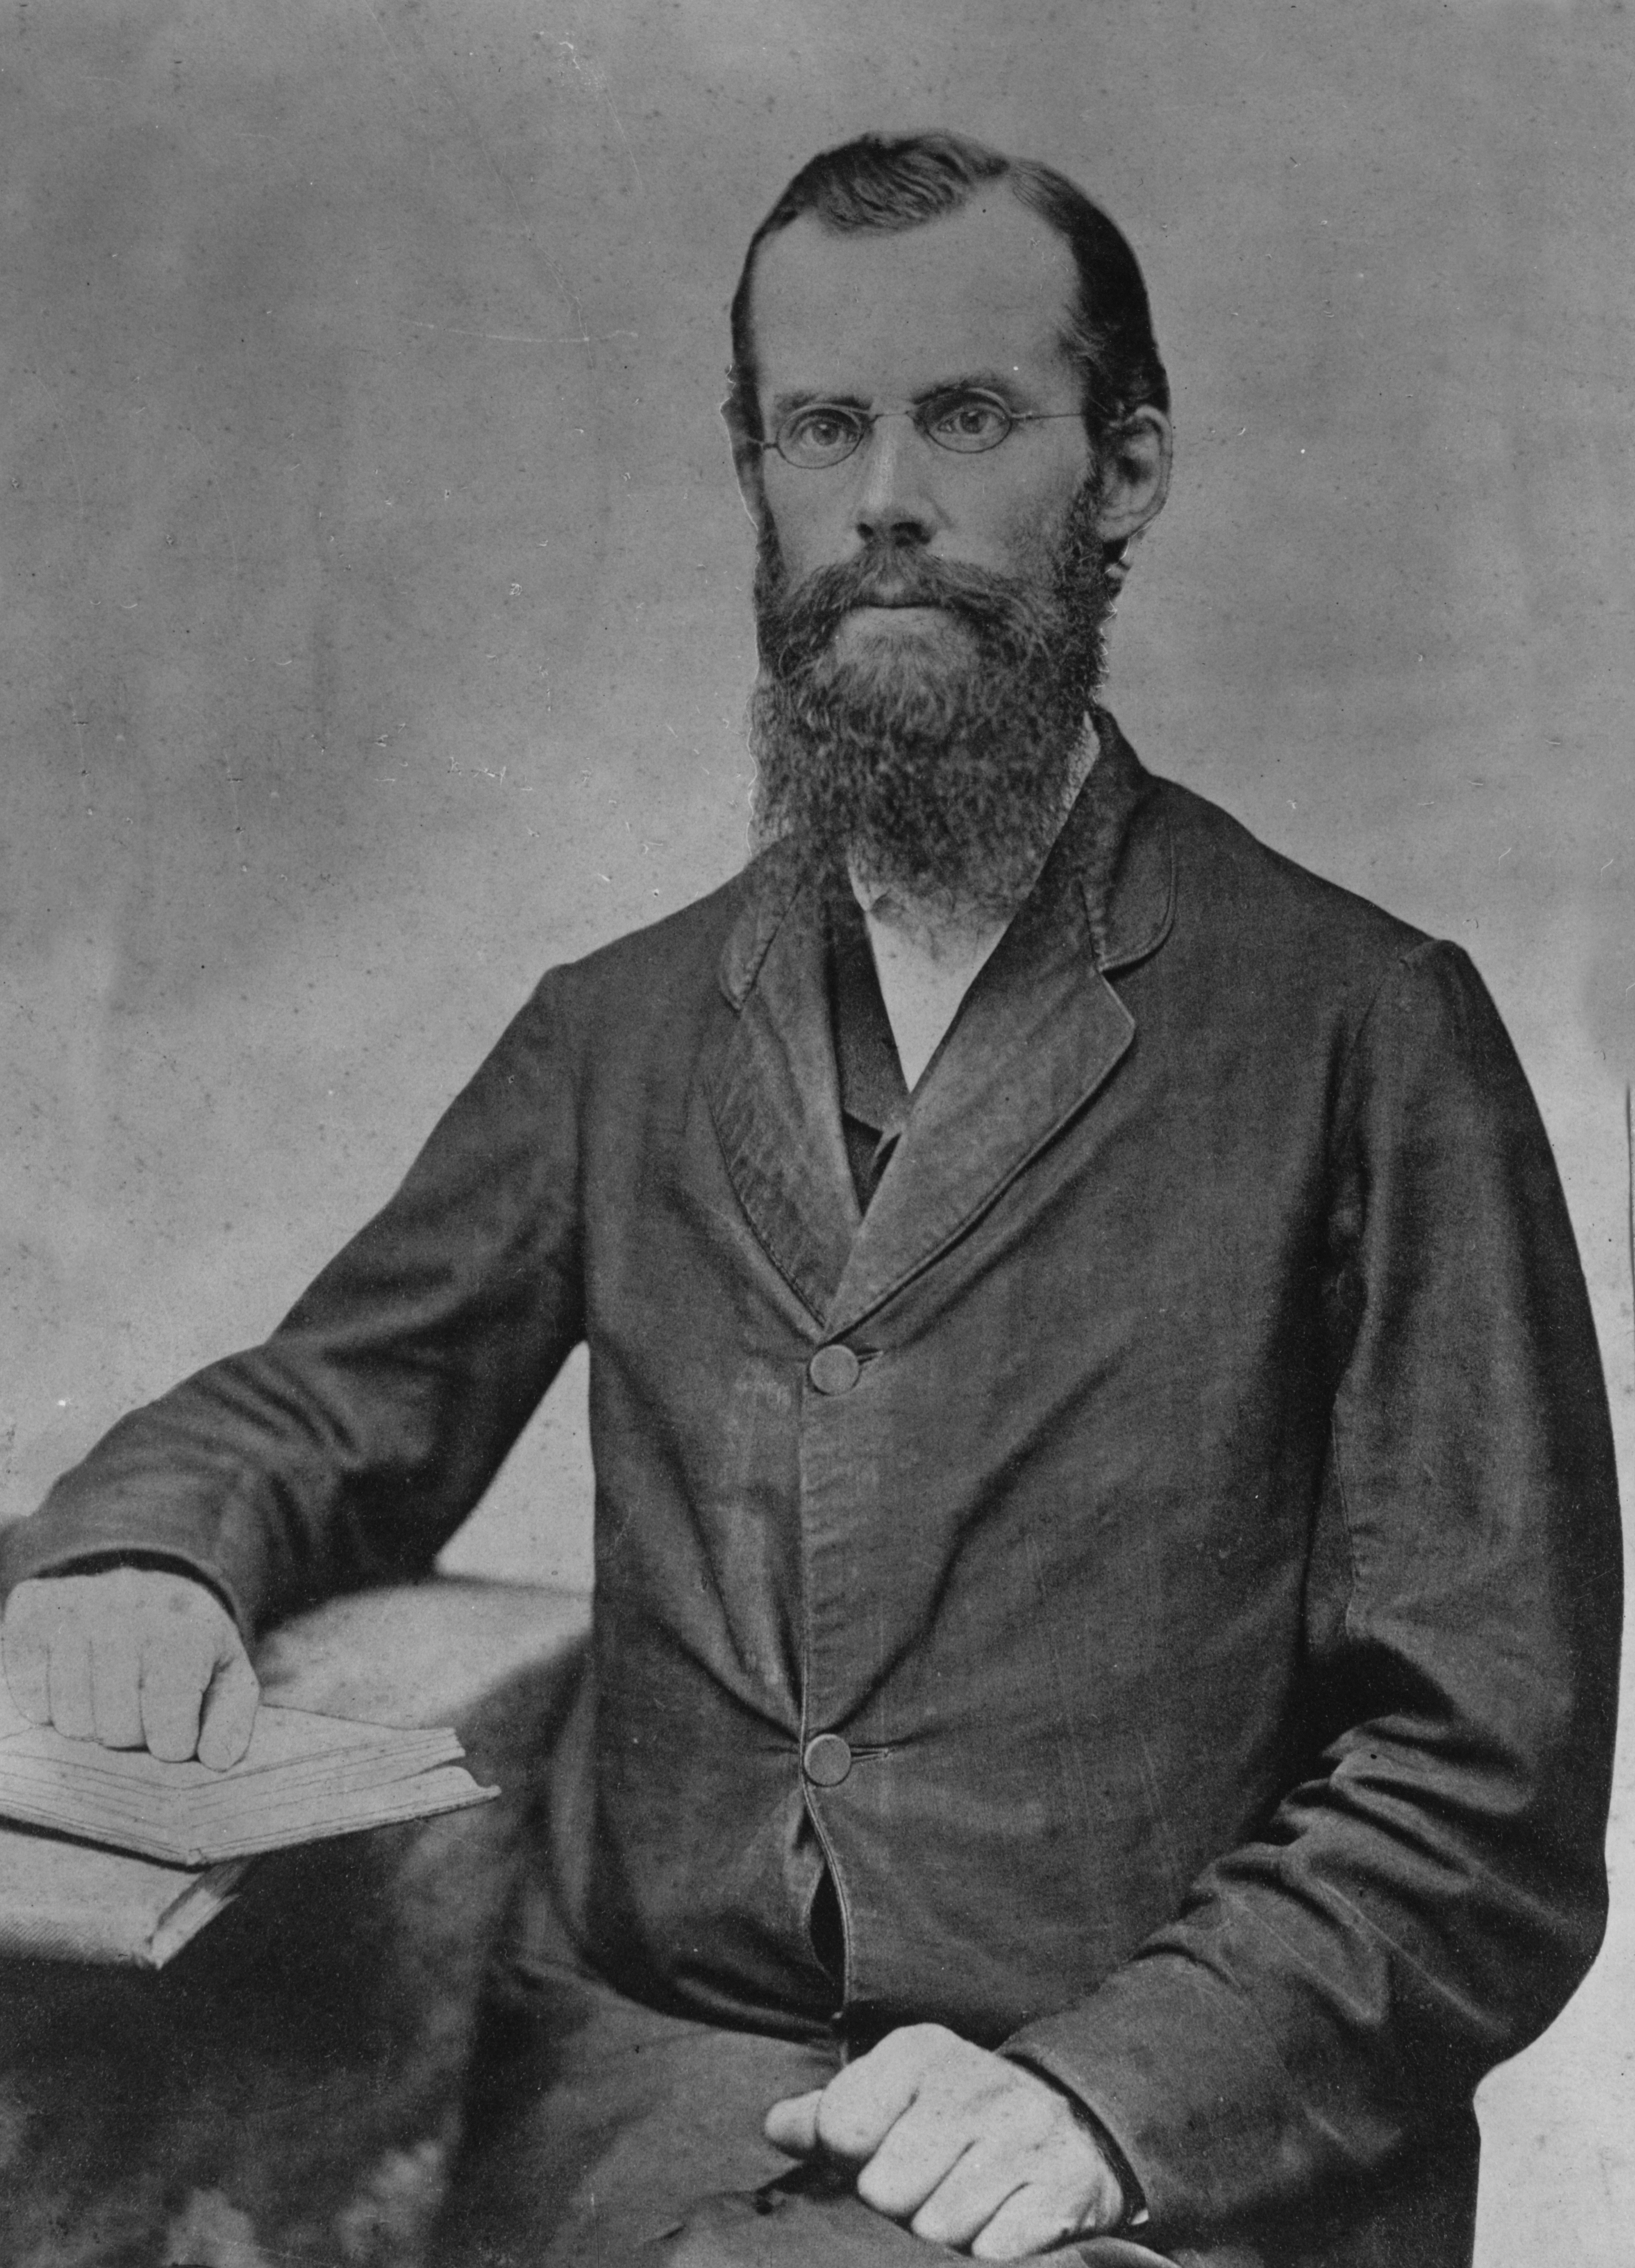
\includegraphics[width=1\linewidth]{images/john-nevins-andrews.jpg}
    \caption*{John Nevins Andrews (1829-1883)}
    \label{fig:j-n-andrews}
\end{figure}


\begin{figure}[hp]
    \centering
    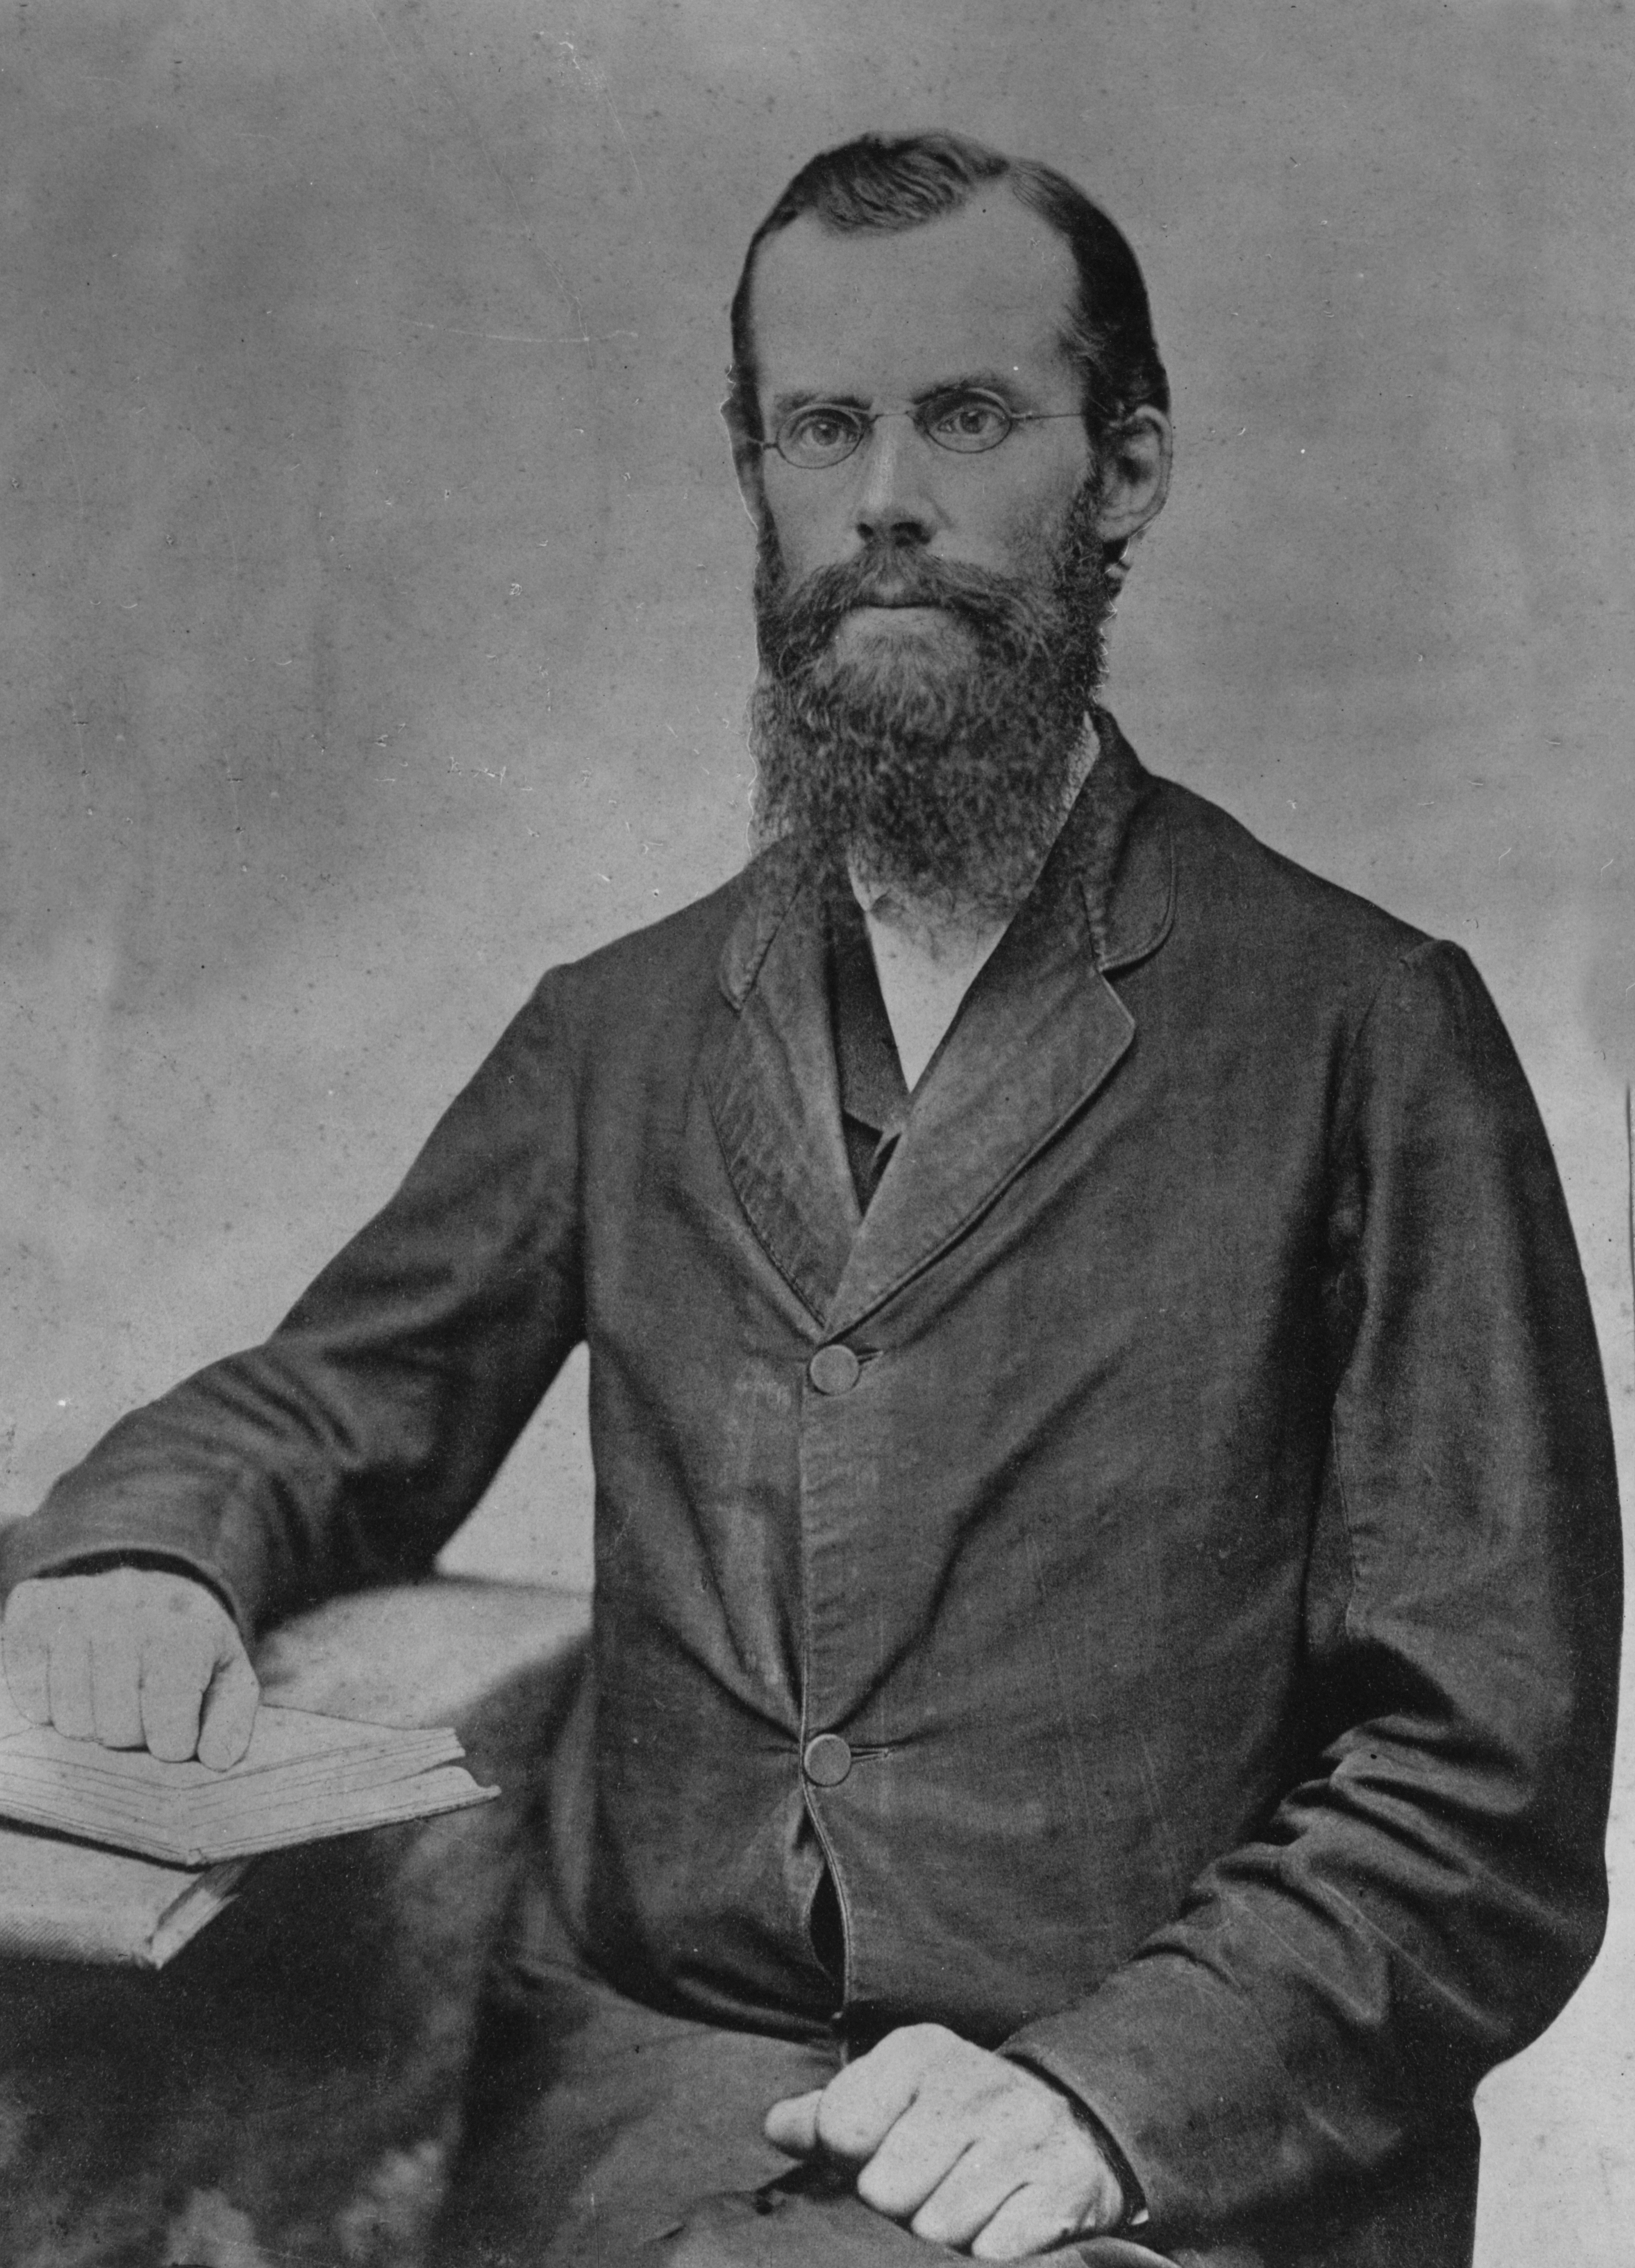
\includegraphics[width=1\linewidth]{images/john-nevins-andrews.jpg}
    \caption*{John Nevins Andrews (1829-1883)}
    \label{fig:j-n-andrews}
\end{figure}


J. N. Andrews said, \others{\textbf{The doctrine of the Trinity which was established in the church by the council of Nicea, A. D. 325}. \textbf{This doctrine \underline{destroys the personality of God, and his Son Jesus Christ our Lord}}...}[John. N. Andrews, The Advent Review and Sabbath Herald, March 6, 1855, p. 185][http://documents.adventistarchives.org/Periodicals/RH/RH18550306-V06-24.pdf]


J. N. Andrews a dit, \others{\textbf{La doctrine de la Trinité qui a été établie dans l'église par le concile de Nicée, en 325 apr. J.-C.} \textbf{Cette doctrine \underline{détruit la personnalité de Dieu, et de son Fils Jésus-Christ notre Seigneur}}...}[John. N. Andrews, The Advent Review and Sabbath Herald, 6 mars 1855, p. 185][http://documents.adventistarchives.org/Periodicals/RH/RH18550306-V06-24.pdf]


In the context of the trinitarian understanding of the \emcap{personality of God}, it is safe to say that the \emcap{personality of God}, or the quality or state of God being a person, in any understanding of Trinity doctrine is a mystery. The problem is that there is no clear view of who is that \textit{one God} who is a person? The underlying claim is made that God is One yet Three, or One in Three; yes, God is a person, and He is one, yet simultaneously He is three persons. This view can never hold any clear perception of the \emcap{personality of God}. Also, it will deny the clearest testimony of the Scriptures that the one God is the Father, and that Christ is truly His only begotten Son. Most trinitarian brothers would agree that Christ is a real and definite being but if a trinitarian were to accept the Father as a real and definite Being, he would also need to accept the Holy Spirit as a real and definite being, thus denying the Holy Spirit as being a \textit{spirit}, the means by which the Father and Son are omnipresent. Conversely, if a trinitarian accepted the Holy Spirit to be a literal spirit, having no body nor form, then he would deny the Father to be a real, definite being. In conversation over the quality or state of God being a person, there is never a clear view of the matter with promoters of the Trinity doctrine; it is subterfuge. \textit{‘Subterfuges’} is a word Sister White used to describe the deception by artifice or stratagem in order to conceal, escape, or evade\footnote{\href{https://www.merriam-webster.com/dictionary/subterfuges}{The Merriam-Webster, ‘subterfuges’} - “\textit{deception by artifice or stratagem in order to conceal, escape, or evade}”} the truth; in other words, something that you cannot grab by head or tail. This is the primary reason Sister White did not engage in the Trinity discussion that would come up in the Seventh-day Adventist Church.


Dans le contexte de la compréhension trinitaire de la \emcap{personnalité de Dieu}, il est juste de dire que la \emcap{personnalité de Dieu}, ou la qualité ou l'état de Dieu d'être une personne, dans toute compréhension de la doctrine de la Trinité est un mystère. Le problème est qu'il n'y a pas de vue claire de qui est ce \textit{Dieu unique} qui est une personne ? L'affirmation sous-jacente est que Dieu est Un mais Trois, ou Un en Trois ; oui, Dieu est une personne, et Il est un, mais simultanément Il est trois personnes. Cette vue ne peut jamais maintenir une perception claire de la \emcap{personnalité de Dieu}. De plus, elle niera le témoignage le plus clair des Écritures que le Dieu unique est le Père, et que Christ est vraiment son seul Fils engendré. La plupart des frères trinitaires seraient d'accord que Christ est un être réel et défini mais si un trinitaire devait accepter le Père comme un Être réel et défini, il devrait aussi accepter le Saint-Esprit comme un être réel et défini, niant ainsi le Saint-Esprit comme étant un \textit{esprit}, le moyen par lequel le Père et le Fils sont omniprésents. Inversement, si un trinitaire acceptait le Saint-Esprit comme étant un esprit littéral, n'ayant ni corps ni forme, alors il nierait que le Père soit un être réel et défini. Dans la conversation sur la qualité ou l'état de Dieu d'être une personne, il n'y a jamais de vue claire de la question avec les promoteurs de la doctrine de la Trinité ; c'est un subterfuge. \textit{‘Subterfuges’} est un mot que Sœur White a utilisé pour décrire la tromperie par artifice ou stratagème afin de dissimuler, échapper ou éviter\footnote{\href{https://www.merriam-webster.com/dictionary/subterfuges}{The Merriam-Webster, ‘subterfuges’} - “\textit{tromperie par artifice ou stratagème afin de dissimuler, échapper ou éviter}”} la vérité ; en d'autres termes, quelque chose que vous ne pouvez saisir ni par la tête ni par la queue. C'est la raison principale pour laquelle Sœur White ne s'est pas engagée dans la discussion sur la Trinité qui surviendrait dans L'Église Adventiste du Septième Jour.


\egw{I was cautioned not to enter into controversy \textbf{regarding the question} that \textbf{\underline{will come up}} over \textbf{these things, because controversy \underline{might lead men to resort to subterfuges, and their minds would be led away from the truth of the Word of God to assumption and guesswork}}. \textbf{The more that fanciful theories are discussed, the \underline{less men will know of God and of the truth that sanctifies the soul}}.}[Lt232-1903.41; 1903][https://egwwritings.org/read?panels=p10197.50]


\egw{J'ai été avertie de ne pas entrer en controverse \textbf{concernant la question} qui \textbf{\underline{surgira}} sur \textbf{ces choses, parce que la controverse \underline{pourrait conduire les hommes à recourir à des subterfuges, et leurs esprits seraient détournés de la vérité de la Parole de Dieu vers des suppositions et des conjectures}}. \textbf{Plus les théories fantaisistes sont discutées, \underline{moins les hommes connaîtront Dieu et la vérité qui sanctifie l'âme}}.}[Lt232-1903.41; 1903][https://egwwritings.org/read?panels=p10197.50]


When we read the works of Seventh-day Adventist pioneers on the \emcap{personality of God}, we see that they did not fall into the Trinity trap. Their non-trinitarian views of God were not due to ignorance, but a knowledge of the truth on the \emcap{personality of God}. They were of keen and noble intellect, understanding the thin line between the truth and error. Their understanding of the \emcap{personality of God} is balanced and solid, strongly supported by the plain and simple “\textit{thus says the Lord}”.


Quand nous lisons les œuvres des pionniers Adventistes du Septième Jour sur la \emcap{personnalité de Dieu}, nous voyons qu'ils ne sont pas tombés dans le piège de la Trinité. Leurs vues non-trinitaires de Dieu n'étaient pas dues à l'ignorance, mais à une connaissance de la vérité sur la \emcap{personnalité de Dieu}. Ils étaient d'un intellect vif et noble, comprenant la ligne mince entre la vérité et l'erreur. Leur compréhension de la \emcap{personnalité de Dieu} est équilibrée et solide, fortement soutenue par le simple et clair “\textit{ainsi dit le Seigneur}”.


Many Adventists today accept the Trinity doctrine because Ellen White supposedly accepted it and promoted it. This is far from the truth and such a conclusion is predicated on lacking knowledge of the Spirit of Prophecy. If anyone was acquainted with the beliefs of Sister White, it was her husband James White. Here is what he has to say about the writings of his wife:


Beaucoup d'Adventistes aujourd'hui acceptent la doctrine de la Trinité parce qu'Ellen White l'aurait supposément acceptée et promue. C'est loin de la vérité et une telle conclusion est fondée sur un manque de connaissance de l'Esprit de Prophétie. Si quelqu'un connaissait les croyances de Sœur White, c'était son mari James White. Voici ce qu'il a à dire sur les écrits de sa femme :


\others{\textbf{We invite all to compare the testimonies of the Holy Spirit through Mrs. W., with the word of God}. \textbf{And in this we do not invite you to compare them \underline{with your creed}}. That is quite another thing. \textbf{\underline{The trinitarian may compare them with his creed, and because they do not agree with it, condemn them}}. The observer of Sunday, or the man who holds eternal torment an important truth, and the minister that sprinkles infants, may each condemn the testimonies’ of Mrs. W. because they do not agree with their peculiar views. And a hundred more, each holding different views, may come to the same conclusion. \textbf{But their genuineness can never be tested in this way}.}[James S. White, The Advent Review, and Herald of the Sabbath, June 13, 1871][https://documents.adventistarchives.org/Periodicals/RH/RH18710613-V37-26.pdf]


\others{\textbf{Nous invitons tous à comparer les témoignages du Saint-Esprit à travers Mme W., avec la parole de Dieu}. \textbf{Et en cela nous ne vous invitons pas à les comparer \underline{avec votre credo}}. C'est tout autre chose. \textbf{\underline{Le trinitaire peut les comparer avec son credo, et parce qu'ils ne s'accordent pas avec celui-ci, les condamner}}. L'observateur du dimanche, ou l'homme qui considère le tourment éternel comme une vérité importante, et le pasteur qui baptise les enfants par aspersion, peuvent chacun condamner les témoignages de Mme W. parce qu'ils ne s'accordent pas avec leurs vues particulières. Et cent autres, tenant chacun des vues différentes, peuvent arriver à la même conclusion. \textbf{Mais leur authenticité ne peut jamais être testée de cette façon}.}[James S. White, The Advent Review, and Herald of the Sabbath, 13 juin 1871][https://documents.adventistarchives.org/Periodicals/RH/RH18710613-V37-26.pdf]


James White was the closest associate of Ellen White, the person who was one with her in God’s uplifting of the Seventh-day Adventist Church. We have a clear and direct testimony from him that Ellen White’s writings are not trinitarian. Today, scholars put a false narrative that Ellen White grew in her understanding of the Trinity doctrine, and eventually accepted and preached it. But we see that Ellen White did not change her standpoint on the \emcap{personality of God} nor did she adhere to the Trinity doctrine. She was unambiguous in her claim that she never did. When the Kellogg crisis came over the \emcap{personality of God}, she remained firm in her view, just as all early Seventh-day Adventist pioneers did—and her dealings with Dr. Kellogg prove that. It is true, the Trinity doctrine \textit{cannot be accepted by those who are loyal to the faith and to the principles that have withstood all the opposition of satanic influences}.\footnote{\egw{Patchwork theories cannot be accepted by those who are loyal to the faith and to the principles that have withstood all the opposition of satanic influences}[Lt253-1903.28; 1903][https://egwwritings.org/read?panels=p14068.9980036]} Today’s official narrative that Ellen White was teaching the Trinity echoes Dr. Kellogg’s claim that the Living Temple taught the same thing as Ellen White. \egwinline{\textbf{But God forbid that this sentiment should prevail}.}[SpTB02 53.3; 1904][https://egwwritings.org/read?panels=p417.272]


James White était le plus proche associé d'Ellen White, la personne qui était une avec elle dans l'élévation par Dieu de L'Église Adventiste du Septième Jour. Nous avons un témoignage clair et direct de lui qu'les écrits d'Ellen White ne sont pas trinitaires. Aujourd'hui, les érudits présentent un faux récit qu'Ellen White a grandi dans sa compréhension de la doctrine de la Trinité, et l'a finalement acceptée et prêchée. Mais nous voyons qu'Ellen White n'a pas changé son point de vue sur la \emcap{personnalité de Dieu} ni n'a adhéré à la doctrine de la Trinité. Elle était sans ambiguïté dans son affirmation qu'elle ne l'a jamais fait. Quand la crise de Kellogg est survenue concernant la \emcap{personnalité de Dieu}, elle est restée ferme dans sa vue, tout comme tous les premiers pionniers Adventistes du Septième Jour l'ont fait—et ses relations avec le Dr Kellogg le prouvent. Il est vrai, la doctrine de la Trinité \textit{ne peut pas être acceptée par ceux qui sont loyaux à la foi et aux principes qui ont résisté à toute l'opposition des influences sataniques}.\footnote{\egw{Les théories de rapiècement ne peuvent pas être acceptées par ceux qui sont loyaux à la foi et aux principes qui ont résisté à toute l'opposition des influences sataniques}[Lt253-1903.28; 1903][https://egwwritings.org/read?panels=p14068.9980036]} Le récit officiel d'aujourd'hui qu'Ellen White enseignait la Trinité fait écho à l'affirmation du Dr Kellogg que Le Temple Vivant enseignait la même chose qu'Ellen White. \egwinline{\textbf{Mais à Dieu ne plaise que ce raisonnement prévale}.}[SpTB02 53.3; 1904][https://egwwritings.org/read?panels=p417.272]


% Adventist pioneers and the Trinity doctrine

\begin{titledpoem}
    \stanza{
        The pioneers stood firm against the Trinity's sway, \\
        Their testimony clear as the light of day. \\
        They saw how this doctrine did subtly disguise, \\
        What Scripture reveals to discerning eyes.
    }

    \stanza{
        James White declared it among "popular fables" found, \\
        A teaching that makes God's personality unsound. \\
        For Father and Son as distinct beings stand, \\
        Not merged into one as the Trinity planned.
    }

    \stanza{
        Two separate persons with purpose aligned, \\
        In spirit and action, united in mind. \\
        Just as disciples in Christ become one, \\
        Yet remain individual under God's Son.
    }

    \stanza{
        The Holy Spirit, God's presence divine, \\
        Not a separate being of the Godhead's design. \\
        But truly God's Spirit sent forth from above, \\
        The Father's representative, agent of love.
    }

    \stanza{
        No Scripture supports what tradition declared, \\
        When at Nicea this doctrine was shared. \\
        John seventeen shatters the trinitarian view, \\
        Revealing the Father and Son as beings true.
    }

    \stanza{
        Christ's divinity rests not in mysterious three, \\
        But in His begotten Sonship we see. \\
        The express image of His Father's face, \\
        Inheriting fullness of divine grace.
    }

    \stanza{
        The pioneers knew what the Bible made clear, \\
        That God is the Father, a Being most dear. \\
        A personal, spiritual presence on high, \\
        Omnipresent through Spirit, yet dwelling on high.
    }

    \stanza{
        So stands the truth against error's long night, \\
        Preserved by the pioneers and Sister White. \\
        Not through confusion or mystical thought, \\
        But through plain Scripture the truth has been taught.
    }
\end{titledpoem}